\documentclass[10pt]{article}
\usepackage[final]{graphicx}
\usepackage{amsfonts}

\topmargin-.5in
\textwidth6.6in
\textheight9in
\oddsidemargin0in

\def\ds{\displaystyle}
\def\d{\partial}

\begin{document}

\centerline{\large \bf Hybrid Splicing of Multi-Scale Downscaler Air Quality Surfaces}

\vspace{.1truein}

\def\thefootnote{\arabic{footnote}}
\begin{center}
  Elizabeth Herman\footnote{Department, University},
  Jeonghwa Lee\footnote{Department, University},
  Kartik Lovekar\footnote{Department, University},
  Dorcas Ofori-Boateng\footnote{Department, University},
  Fatemeh Norouzi\footnote{Department, University},
  
  Benazir Rowe\footnote{Department of Mathematical Sciences, University of Nevada Las Vegas},
  Jianhui Sun\footnote{Department, University}
\end{center}

%\vspace{.1truein}

\begin{center}
Problem presenters: Elisabeth Mannshardt\footnote{Environmental Protection Agency}, Barron Henderson\footnote{Environmental Protection Agency}, and Brett Gantt\footnote{Environmental Protection Agency}

 
Faculty Mentor: Brian Reich\footnote{NCSU Statistics}
\end{center}


\vspace{.3truein}
\centerline{\bf Abstract}

\begin{itemize}
\item Summarize the results presented in the report, and the contributions
of your research.

\item Readers should not have to look at the rest of the paper in order to 
understand the abstract.

\item Keep it short and to the point.
\end{itemize}

\section{Introduction}



To differentiate two different region divisions in this study, nine climatically consistent regions within the contiguous United States will be referred to nine NOAA regions hereafter, which include Northwest (NW), Northern Rockies and Plains (NR), West (W), Southwest (SW), Upper Midwest (UM), South (S), Ohio Valley (OV), Southeast (SE), and Northeast (NE), while nine square regions, each covers one NOAA region, constituted by grid cells, on which Downscaler model is calculated, will be referred to as DS regions. Each NOAA region includes several spatially adjacent states and they do not intersect with each other, while on the other hand, pair of adjacent DS regions, in order to completely cover their corresponding NOAA regions, share an area of intersection. Hence, for each AQS monitoring station which locates in the intersection of two DS regions,the grid cells which it belongs to, will simultaneously have two different mean DS estimates and standard error estimates.  DS model is applied on regional scale (DS regions) producing 9 surfaces of estimate $PM_{2.5}$. It was seen that the DS estimated surfaces of $PM_{2.5}$  are not smoothly connected. Especially the DS estimates from the region NW and NR are so different on the boundary that it leaves an issue of creating smooth surface.

To tackle this issue, we use the grid cells that lie inside the overlap areas of the region (2-4 overlaps per region). we use model averaging  where the probability density fucntion of a grid cell in the overlap   is a weighted average of density functions,  which are the predictive distributions of the grid cell from regional DS. We set the weight proportional to the distance of the grid cells to the boundary of the overlap, because the larger the distance is, the further the point is toward the inner area and less influenced by adjacent region.

The parameter $\phi$ is also introduced to adjust the effect of distance on wieghts. More specifically, we have the following weight for the density function from region $i$ with point $s$ :
$$  w_{i}(s)=\exp(-\phi ds_i) $$  where $ds_i $ is the  distance of point s to outer boundary of region $i$. This implies that the larger the $\phi$ is, the bigger influence the distance has on the wieght. In extream case when $\phi$ is zero , the weight are simply evenly distrubuted among the densities, and if $\phi=\infty$  the probability density function simply becomes the closest density function and the weight has no effect on averaging.

Data strategy overview:
1.    Find the grid cells that lie inside the overlap areas of the region (2- 4 overlaps per region)
2.    Find downscaler prediction of mean and variance for each grid cell in the overlap.
3.    For AQS stations inside the overlap, find the grid cell it’s located in.
4.    For each AQS station inside the overlap combine the following info that will be used in the model: AQS reading, DS mean 1, DS mean 2, DS Standard Deviation 1, DS Standard Deviation 2, distance to the boundary of zone 1, distance to the boundary of zone 2.





For AQS stations inside the overlap,we find the grid cell it’s located in and we calculate "d" as the "distance to the bounday of "zone 1" to the "zone n" based on our number of zones in the overlapping area of each region. Then, we will Find downscaler prediction of mean ("mu") and standard deviation ("sd") for each grid cell in the overlap.
for instance, as we have two zones of NW and NR, we want to optimize the maximum likelihood function of each zone regarding normal distribution and then, to consider the probability density function regarding the average modeling of 2 (in general n) normal distribution of 2 zones in a region.
At the end, based upon the MLE function, we can figure out "phi" as a parameter to see that the overlap intersection part goes to which zone!


========================================================================================







you can ignore the below














To differentiate two different region divisions in this study, nine climatically consistent regions within the contiguous United States would be referred to nine NOAA regions hereafter, which include Northwest (NW), Northern Rockies and Plains (NR), West (W), Southwest (SW), Upper Midwest (UM), South (S), Ohio Valley (OV), Southeast (SE), and Northeast (NE), while nine square regions, each covers one NOAA region, constituted by grid cells, on which Downscaler model is calculated, would be referred to as DS regions. Each NOAA region includes several spatially adjacent states and they do not intersect with each other, while on the other hand, pair of adjacent DS regions, in order to completely cover their corresponding NOAA regions, shares an area of intersection. Hence, for each AQS monitoring station which locates in the intersection of two DS regions, the grid cell it belongs to will simultaneously have two different mean DS estimates and standard error estimates. Finding a justifiable approach to combine mean/standard error from two regions is of main interest in this study.

Based on the data that we have for the intersection of NW and NR, we consider "Y" as the number of grid cells in each region. "mu" is the mean prediction of the intersection between AQS and DS grids and also, "sd" in the standard deviation of the intersection between AQS and DS grids. Besides, we have "d" as a matrix of distance.
As we have two zones of NW and NR, we want to optimize the maximum likelihood function of each zone regarding normal distribution. we specify a weighted average considering a "phi" to each normal distribution.
At the end, based upon the MLE function, we can consider "phi" as a parameter to see that the overlap intersection part goes to which zone!

Data strategy overview:
1.    Find the grid cells that lie inside the overlap areas of the region (2- 4 overlaps per region)
2.    Find downscaler prediction of mean and variance for each grid cell in the overlap.
3.    For AQS stations inside the overlap, find the grid cell it’s located in.
4.    For each AQS station inside the overlap combine the following info that will be used in the model: AQS reading, DS mean 1, DS mean 2, DS Standard Deviation 1, DS Standard Deviation 2, distance to the boundary of zone 1, distance to the boundary of zone 2.

It was seen from the 9 overlapping NOAA sufaces from regional DS that the
predictive models are not smoothly connected.
 Especially in the north west  and west north central  regions, the predictive values on the boundary are so different that it leaves an issue of creating smooth surface.
To tackle this issue, we use averaging model where the density fucntion of a point in the overlaping region  is a weighted
average of density functions,  which are the original predictive 
distributions of the point from regional DS.
We set the weight proportional to the distance between the point and the boundary of the outer region(outer region refers to the ..), because the larger the distance is, the further the point is toward the inner area and less influenced by adjacent region.  
We also introduce the parameter $\phi$ to adjust the effect of distance on wieghts. More specifically, we have the following weight for the density function from region $i$ with point $s$ :
\[  w_{i}(s)=\exp(-\phi ds_i) \]  where $ds_i $ is the  distance of point s to outer boundary of region $i$.
This implies that the larger the $\phi$ is, the bigger influence the distance has on the wieght. In extream case when $\phi$ is zero , the weight are simply evenly distrubuted among the densities, and if $\phi=\infty$  the density function simply becomes the closest density function and the weight has no effect on averaging. 

+++++++++++++++++++++++++++++++++++++++++++++++++++++++++++++++++++++++++++++++++++++++++++++


To differentiate two different region divisions in this study, nine climatically consistent regions within the contiguous United States will be referred to nine NOAA regions hereafter, which include Northwest (NW), Northern Rockies and Plains (NR), West (W), Southwest (SW), Upper Midwest (UM), South (S), Ohio Valley (OV), Southeast (SE), and Northeast (NE), while nine square regions, each covers one NOAA region, constituted by grid cells, on which Downscaler model is calculated, will be referred to as DS regions. Each NOAA region includes several spatially adjacent states and they do not intersect with each other, while on the other hand, pair of adjacent DS regions, in order to completely cover their corresponding NOAA regions, share an area of intersection. Hence, for each AQS monitoring station which locates in the intersection of two DS regions,the grid cells which it belongs to, will simultaneously have two different mean DS estimates and standard error estimates.  DS model is applied on regional scale (DS regions) producing 9 surfaces of estimate $PM_{2.5}$. It was seen that the DS estimated surfaces of $PM_{2.5}$  are not smoothly connected. Especially the DS estimates from the region NW and NR are so different on the boundary that it leaves an issue of creating smooth surface.

To tackle this issue, we use the grid cells that lie inside the overlap areas of the region (2-4 overlaps per region). we use model averaging  where the probability density fucntion of a grid cell in the overlap   is a weighted average of density functions,  which are the predictive distributions of the grid cell from regional DS. We set the weight proportional to the distance of the grid cells to the boundary of the overlap, because the larger the distance is, the further the point is toward the inner area and less influenced by adjacent region.

The parameter $\phi$ is also introduced to adjust the effect of distance on wieghts. More specifically, we have the following weight for the density function from region $i$ with point $s$ :
$$ w_{i}(s)=\exp(-\phi ds_i) $$  where $ds_i $ is the  distance of point s to outer boundary of region $i$. This implies that the larger the $\phi$ is, the bigger influence the distance has on the wieght. In extream case when $\phi$ is zero , the weight are simply evenly distrubuted among the densities, and if $\phi=\infty$  the probability density function simply becomes the closest density function and the weight has no effect on averaging.

Data strategy overview:
1.    Find the grid cells that lie inside the overlap areas of the region (2- 4 overlaps per region)
2.    Find downscaler prediction of mean and variance for each grid cell in the overlap.
3.    For AQS stations inside the overlap, find the grid cell it’s located in.
4.    For each AQS station inside the overlap combine the following info that will be used in the model: AQS reading, DS mean 1, DS mean 2, DS Standard Deviation 1, DS Standard Deviation 2, distance to the boundary of zone 1, distance to the boundary of zone 2.





For AQS stations inside the overlap,we find the grid cell it’s located in and we calculate "d" as the "distance to the bounday of "zone 1" to the "zone n" based on our number of zones in the overlapping area of each region. Then, we will Find downscaler prediction of mean ("mu") and standard deviation ("sd") for each grid cell in the overlap.
for instance, as we have two zones of NW and NR, we want to optimize the maximum likelihood function of each zone regarding normal distribution and then, to consider the probability density function regarding the average modeling of 2 (in general n) normal distribution of 2 zones in a region.
At the end, based upon the MLE function, we can figure out "phi" as a parameter to see that the overlap intersection part goes to which zone!






















   
It should be written as much as possible in non-technical terms, so that a
lay reader can understand the context and the contribution of the paper.

\begin{itemize}
\item Describe the problem you are trying to solve, the approach
you took, and summarize your contribution and results.

\item Review the history of this problem, and existing literature.

\item Give an outline of the rest of the paper.
\end{itemize}

\section{The Problem}
\begin{itemize}
\item Give a precise technical description of your problem. 

\item State and justify all your assumptions. 

\item Define notation. 

\item Describe your data, how you collected them, their properties,
and whether you did 
anything to them (removed noise, filled in missing data, 
applied normalizations).
\end{itemize}
The data we will be using to generate our results comes from three sources, AQS sites, IMPROVE sites, and evaluations of the Downscaler model.  The data we looked at was data collected in Quarter 1.  That is, the data we are considering was collected in January, February, and March.  The methodology we will develop below can be extended to any quarter of the year.  Below, we will discuss how the data source is collected, why the data source is beneficial, and the limitations we have using the data.  We will begin with the data collected at the AQS sites.  

The AQS data was collected at AQS sites.  These sites have AQS machines on the ground to collect concentrations of pollutants (specifically PM-25, the pollutant we are interested in).  We will henceforth refer to this data as "AQS data" or "the ground truth."  While we do have actual readings of the concentration of PM-25, this data is usually only collected near large cities.  The reason for this is that there is legislation that requires cities of certain populations to purchase a machine and then use it to collect readings ofs pollution in the air.  Additionally, the data is not collected every day.  For example, there are locations that collect data every 6 six days.  As a result, it is difficult to get a consistent amount of reliable data from these machines.  Note also that we are not considering the effects of noise in data collection (i.e. no measurement noise in our data collection).

Our second source of data comes from IMPROVE sites.  These sites are again measuring the concentration of the pollutant PM-25 in the air.  Unlike the AQS sites, these sites are located in areas in which there is not a high concentration of the pollutant.  For instance, the IMPROVE sites can be located in a National Park or other rural areas.

Our last piece of data we will be using is from a model called Downscaler (DS).  This model works on a grid, the continental United States divided into 12km by 12km pieces.  It essentially uses a "fancy" linear regression to incorporate the data gathered from the AQS sites and another source of information that indicates the type of environment the grid block is located at.  The output of Downscaler is a mean and standard error for each grid point.  Because the Downscaler is an evaluation of a model, we can choose the area in which we run the model.  This is the source of our problem.  Normally, the Downscaler is ran on a national scale.  That is, it incorporates all of the data from the AQS sites located in the continental United States.  The potential problem with this, is that if the location we are trying to extrapolate is in the NW, the model considers the readings of the AQS machines in the SE.  The hypothesis is that while there is some correlation between the regions in close proximity to each other, overall, the concentrations of PM-25 on one side of the country do not have an effect on the readings on the other side of the country.  The proposed solution is to run the Downscaler on a regional scale with overlapping areas in-between the regions.  That way, a specific grid point only includes information that is "relevant" to the region that it is in.  We include an overlap region because it is assumed that the grid points on the edge of the boundary will be impacted by the near-by grid points in the adjacent region.  Two questions arise from this proposed solution: what regions should be used? and how do we deal with the overlapping region?.

We will address the first question by splitting the continental United States by the NOAA climate zones.  This means that we will have nine regions that we are running the Downscaler on.  The nine regions are Northwest (NW), North Rockies (NR), Upper Midwest (UM), Ohio Valley (OV), Northeast (NE), Southeast (SE), South (S), Southwest (SW), and West (W).  Recall that we are considering these zones plus some overlap into the adjacent regions.  Figure \ref{US} shows the continental US broken up into the NOAA Climate Zones.

% % % %WE STILL NEED TO CITE THIS!!!!!!!!!!!!!!!!!!!
\begin{figure} %[!h]
\begin{center}
  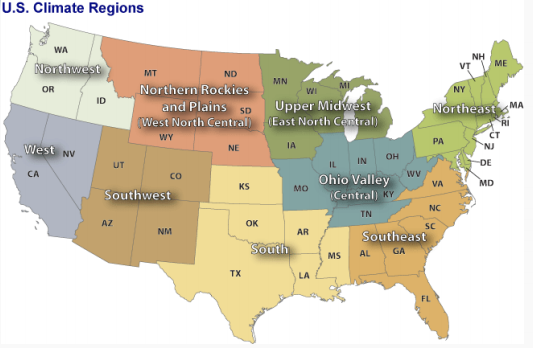
\includegraphics[width=3.9in]{ContUS.png}
\end{center}
\vspace{-0.15truein}
\caption{NOAA Climate Zones.}
\label{US}
\hspace{1.70in}
\vspace{-0.15truein}
\end{figure}

The second question is the reason for which we are writing this paper.  Because we are running the Downscaler for each region plus some overlap, The overlap area will have two (or more) DS values for which the Downscaler model provides an evaluation at each gridpoint.  This paper seeks to provide a methodology for this overlap region.  An example of the overlap region is provided in Figure \ref{overlap}.  Notice that the boxes represented by the dashed lines are the NOAA Climate Zones, i.e. they are a collection of states defined by NOAA in which the states have similar climates.  The two regions that we ran Downscaler on are represented by the solid lines.  By running the Downscaler twice, in the overlap region (which includes the NOAA Climate Zone boundary) we have an evaluation of Downscaler at each grid point.  As a result, we need to find a way to combine the two evaluations into one that makes sense for the grid point.

\begin{figure} %[!h]
\begin{center}
  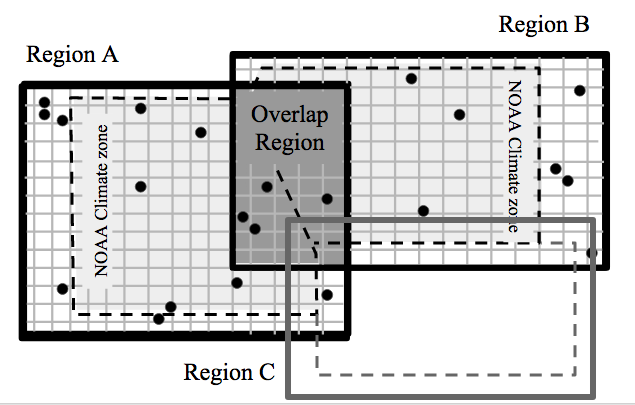
\includegraphics[width=5.9in]{overlap.png}
\end{center}
\vspace{-0.15truein}
\caption{Overlap region on NOAA Climate Zones.}
\label{overlap}
\hspace{1.70in}
\vspace{-0.15truein}
\end{figure}

\section{The Approach}
\begin{itemize}
\item Present and justify your approach for solving the problem. 
\item Explain the advantages of your approach over existing ones.

\item Tell a story.
Don't just say: ``I did this, then I did this, and at last I did this''.
\end{itemize}

\section{Computational Experiments}
Give enough details so that readers can duplicate your experiments.

\begin{itemize}
\item Describe the precise purpose of the experiments, and what they 
are supposed to show.

\item Describe and justify your test data, and any assumptions you made to 
simplify the problem.

\item Describe the software you used, and the 
parameter values you selected.

\item 
For every figure, describe the meaning and units of the coordinate axes, 
and what is being plotted.

\item Describe the conclusions you can draw from your experiments
\end{itemize}

\section{Summary and Future Work}
\begin{itemize}
\item Briefly summarize your contributions, and their possible
impact on the field (but don't just repeat the abstract or introduction).
\item Identify the limitations of your approach.
\item Suggest improvements for future work.
\item Outline open problems.
\end{itemize}



\end{document}
